
\section{Problem Formulation}
\label{sec:ProblemFormulation}

We consider a resource deployment problem in a virtualized network infrastructure, such as a data center, where the virtualized resources can be leased with reliability guarantees. Each resource lease request is modeled as undirected graph $G=(N,E,S)$. N is a set of compute nodes, E is a set of edges and S is a partial set of service functions. We call this a virtual network(VN).



\subsection{Reliability,Survivable}
Reliability is guaranteed on the set of critical nodes $C\subset N$ of a VN through redundant virtual nodes with backup nodes set $B(V,S)$. A backup (redundant) node b must be able to assume full execution of a failed critical node c. Hence, the backup node must have sufficient resources in terms of computation


\subsection{How many backups?}
The number of redundant nodes depend on the physical mapping, and the failure models of both the physical nodes and the virtual infrastructure.

The problem is to  allocate least resources for a VN $G$,including redundancy such that a reliability guarantee of at least r is achieved. 

\subsection{Node-Fault Graph}
\subsubsection{NFT}
We refer to the concept of k-NFT\cite{harary1996node}. Let $G(V,E)$ be a graph with $n$ nodes and $q$ edges. An
(n+k)-node graph $G^*$ is k-node fault-tolerant, or k-NFT, with respect to $G$ if every graph $G^*-R$ obtained by removing any nodes set $R$ of $k>0$ nodes from $G^*$ contains $G$. Generally speaking, $G$ is subgraph isomorphism of $G^*-R$. We will refer to $G^*$ as a k-NFT supergraphs of $G$ or simply as a k-NFT($G$). We also say $G^*\cong$ k-NFT($G$), the set of all k-NFT($G$) supergraphs of $G$. The complete graph $K_{n+k}$ of $n + k$ nodes is trivially a k-NFT supergraph of every $G$ that contains up to n nodes. We are concerned mainly with k-NFT graphs that satisfy the following optimality criterion: If $G^*$ has the smallest number $|E(G^*)|$ of edges among all (n + k)-node supergraphs that are k-NFT with respect to $G$, then $G^*$ is optimally k-NFT with respect to $G$. The number $NFT_{ec}$(G,k) =$|E(G^*)-E(G)|$ is called the k-NFT edge cost of G. The number $NFT_{nc}$(G,k) =$|V(G^*)-V(G)|$ is called the k-NFT node cost of G, however $NFT_{nc}$(G,k) = k with respect with k node fault tolerant graph of graph $G$ .
\subsubsection{SNFT}
When every nodes of graph $G(V,E,S)$ have a specific flags set $S$(corresponding to service functions) and every nodes is marked by only one specific flag, which is denoted by node flag. An (n+k)-node graph $G^o$ is k-specific node fault tolerant, or k-SNFT, with respect to $G(V,E,S)$ if every graph $G^o-R$ obtained by removing any nodes set $R$ of $k>0$ nodes from $G^o$ contains $G$, $G$ is subgraph isomorphism of $G^o-R$ and the node flag of any nodes $n$ of $G$ belong specific flags set of node $n^o$ corresponding to node $n$. We will refer to $G^o$ as a k-SNFT supergraphs of $G$ or simply as a k-SNFT($G$). The number $SNFT_{nc}$(G,k) =$|V(G^o)-V(G)|$ is called the k-SNFT node cost of G. The number $SNFT_{ec}$(G,k) =$|E(G^o)-E(G)|$ is called the k-SNFT edge cost of G.
\subsubsection{SNFT with B}
After our simple inference, if we set the $SNFT_{nc}$(G,k) is the main cost than edge cost, the number of $SNFT_{nc}$(G,k) must equal k, moreover the added node could have any specific flags. but the added node should be limited in specific flags set after our analyzing the real-world practical phenomenon.

Suppose added nodes is from backup nodes set $B(V,S)$, where every nodes of backup nodes set $B$ have a specific flags set. The k-SNFT($G,B$) is that requesting a k specific node fault tolerant graph of graph $G$ and added nodes belong backup nodes set $B$.

%The limited node of $G^o-G$ with respect to any $G^o$ is used as inserted node from specific node set $B$ which is premise. k-specific node fault-tolerant graph of $G$ with limit-inserted node set $B$ is denoted by k-SNFT($G,B$).

\subsection{Survivable Virtual Network Request}
%When a survivable request of virtual network is coming, survivable virtual network requests are associated with node's service functions.
In any real virtual networks, any nodes of virtual network  are deployed with a service function and the physical node could run some various service functions. After virtual network VN is embedded into substrate network, a node of virtual network could fail so that we should obtain survivable VN to be embedded into substrate network so that recovery from the failure even though one node of virtual network failed. The added nodes of survivable virtual network are embedded into substrate network ultimately, the added nodes have specific service functions similarly.



There are different combinations of service function in any nodes of virtual network, and there is only one type of service function running on the corresponding virtual node at that moment.

There exist many backup virtual nodes $B(V,S)$ for guaranteing maintaining former topological structure of virtual network request $G(V,E,S)$ once one fault node $v$ appeared in virtual network request $G(V,E,S)$. Solving the survivable request of virtual network is of equivalence with asking 1-SNFT(G,B) of graph $G$ and backup nodes set $B$.

An example of a typical survivable request of virtual network is show in Fig.\ref{fig:svnr}.
\begin{figure}
\centering
% Requires \usepackage{graphicx}
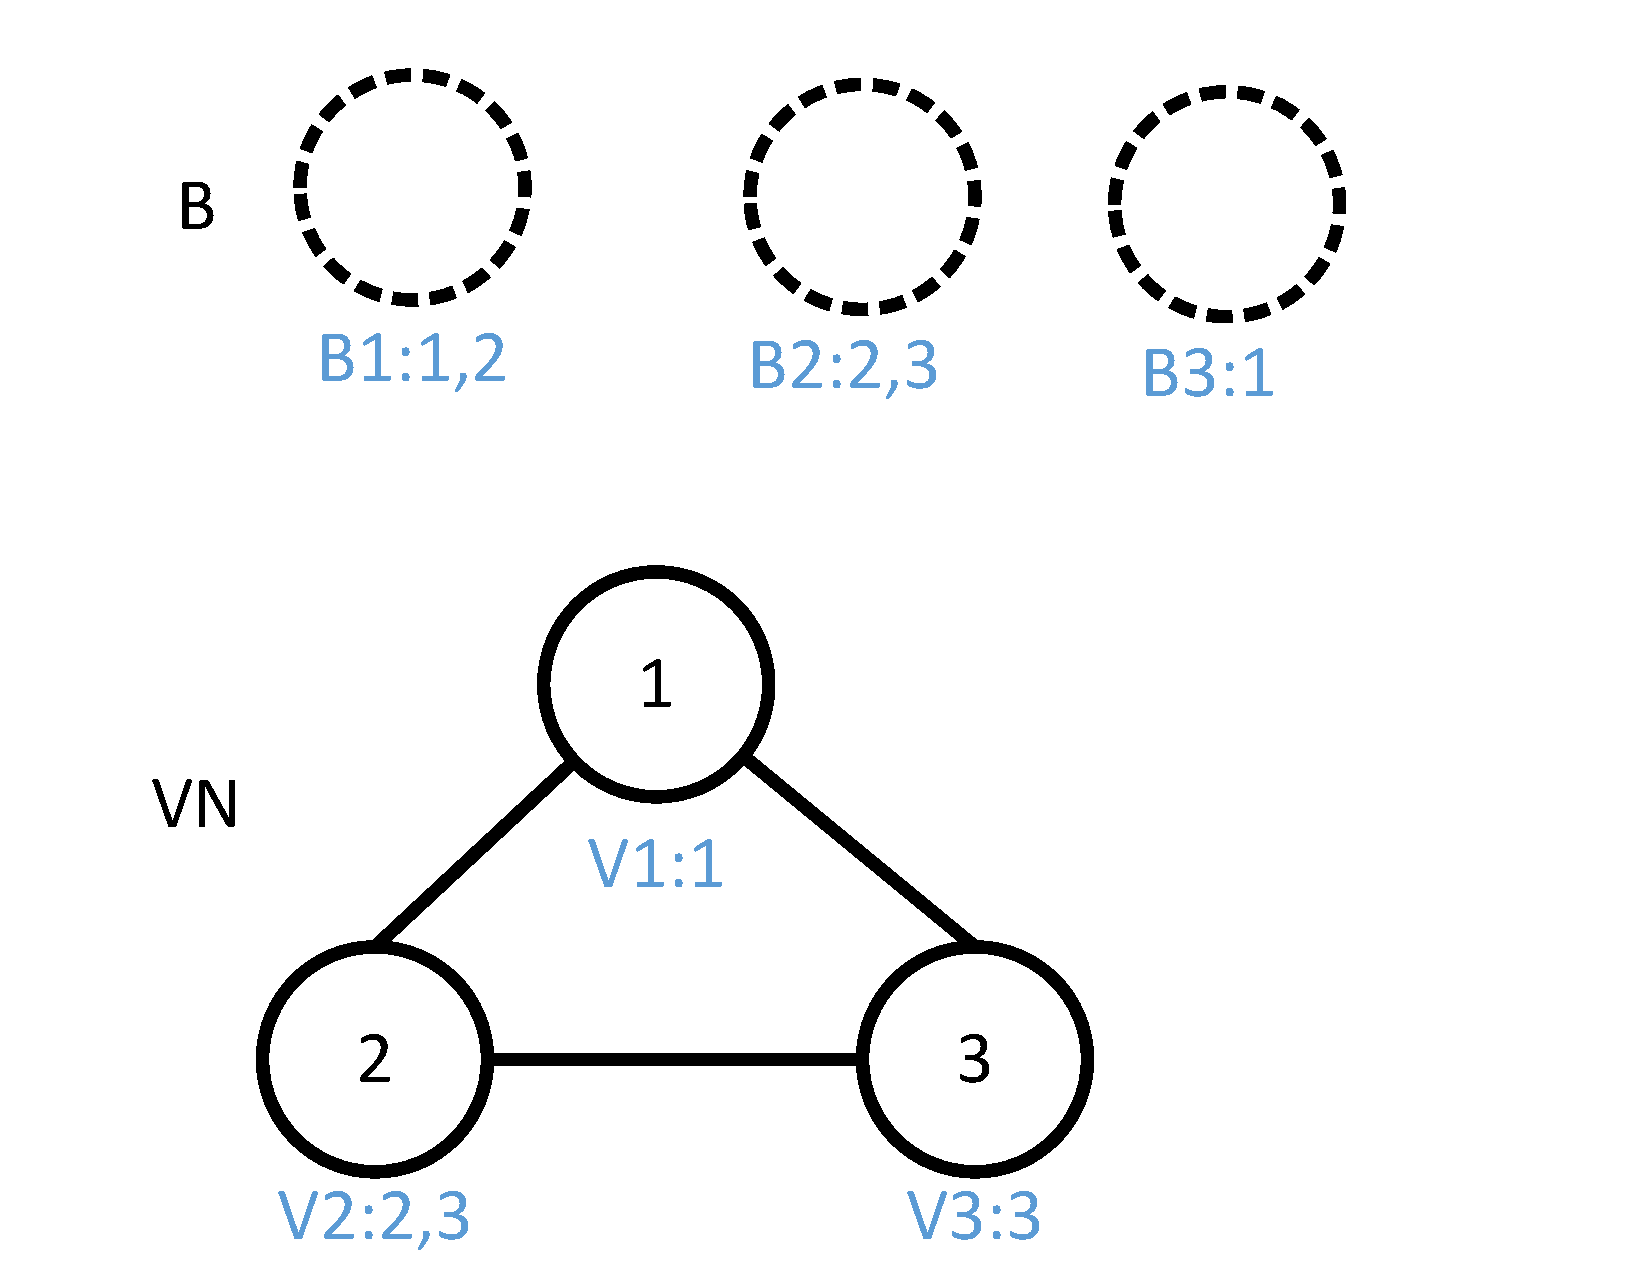
\includegraphics[width=1.5in]{Fig/SVNR}\\
\caption{SVNR}\label{fig:svnr}
\end{figure}

Generally speaking, survivable request of virtual network is 1-specific node fault-tolerant of virtual network $G(V,E,S)$ with backup nodes set $B(V,S)$. Inserting any edges among nodes $V\cup B$ to construct $G^o$ as shown in Fig.\ref{fig:optgraphsvnr},\ref{fig:nonoptgraphsvnr}, for which G is a subgraph of $G^o-v(\forall v\in V\cup B^o,B^o\subset B)$.
%$G^o$([1-SNFT(G),B]) is survivable virtual network $SVN$.(one node of backup nodes n failed, )

\subsection{reduce immigration when node fail}
However, this poses a limitation since the result only guarantees graph isomorphism and not equality. In other words, there may be a need to physically swap remaining VMs while recovering from some failure in order to return to the original infrastructure G. Recovery may then be delayed, or require more resources for such swapping operations.

\begin{figure}
\centering
% Requires \usepackage{graphicx}
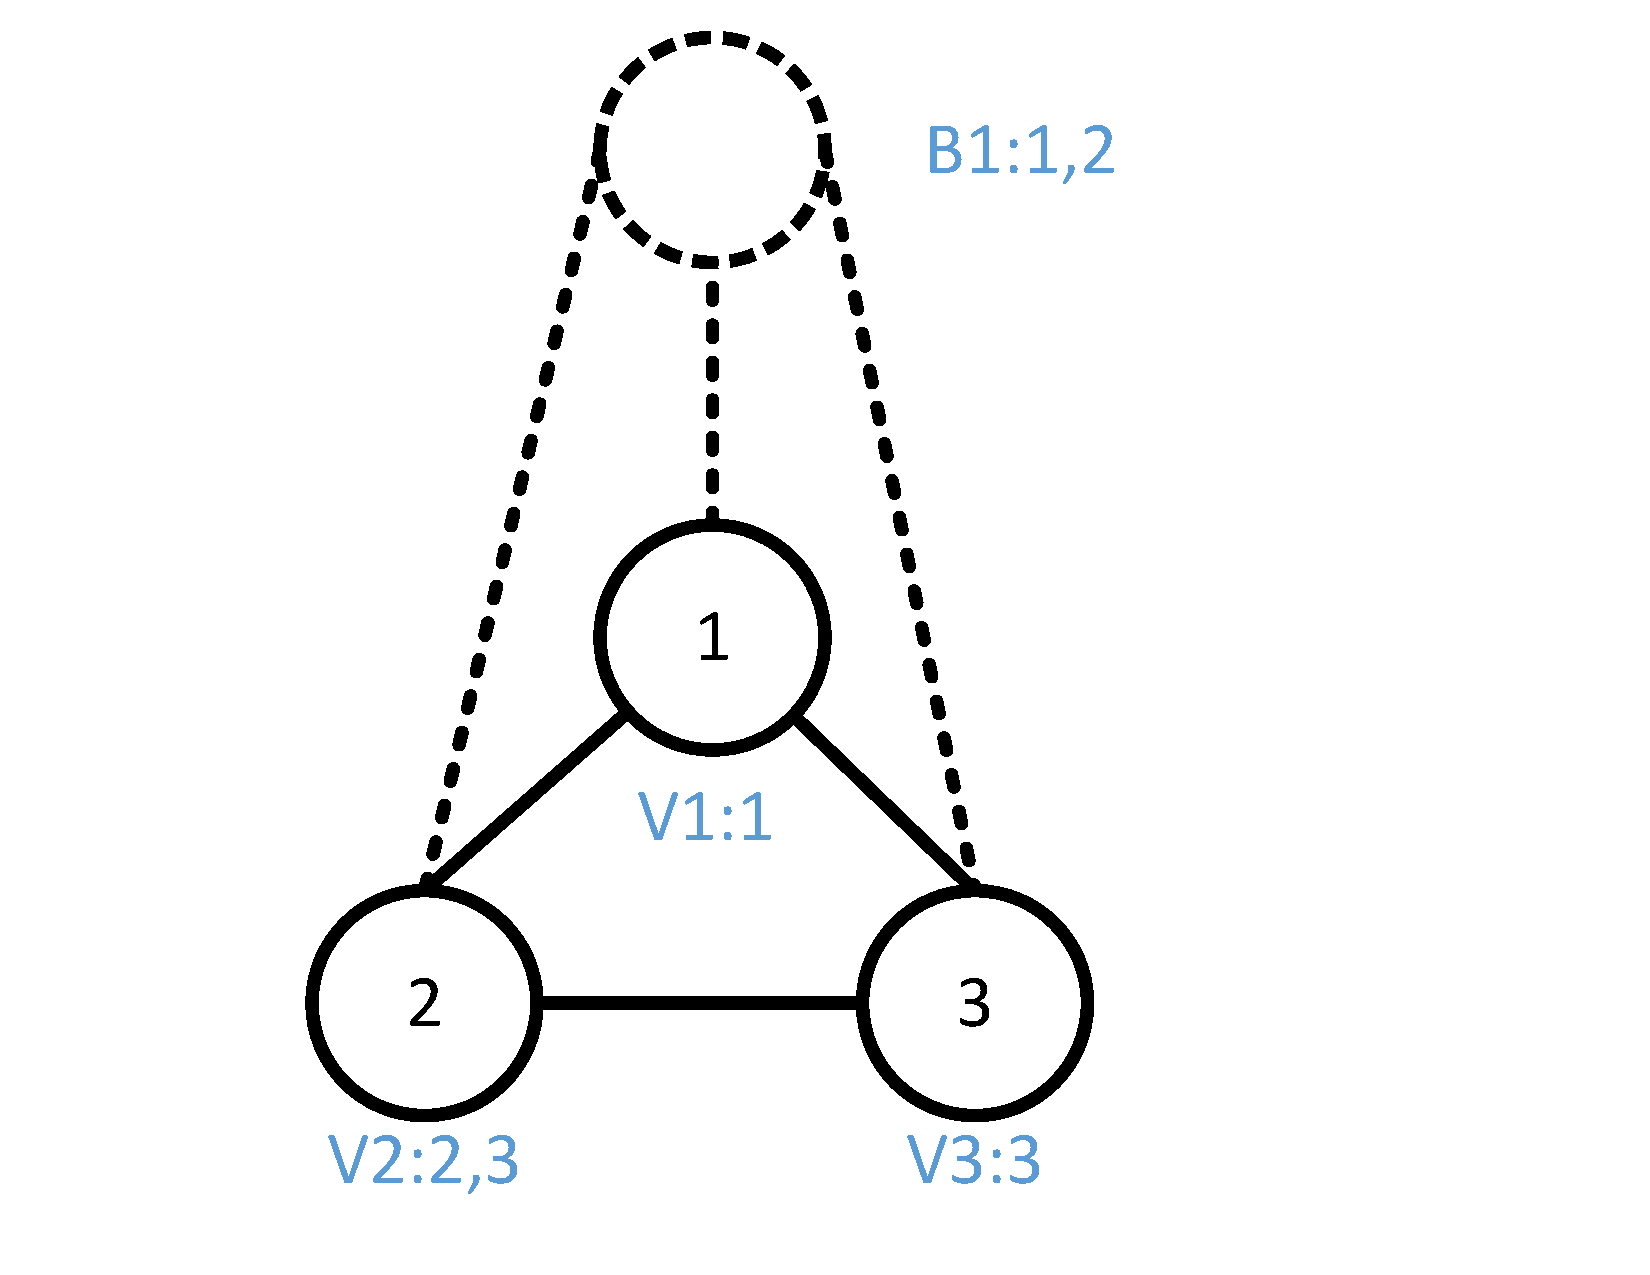
\includegraphics[width=1.5in]{Fig/optgraph_SVNR}\\
\caption{optimal SVNR}\label{fig:optgraphsvnr}
\end{figure}
\begin{figure}
\centering
% Requires \usepackage{graphicx}
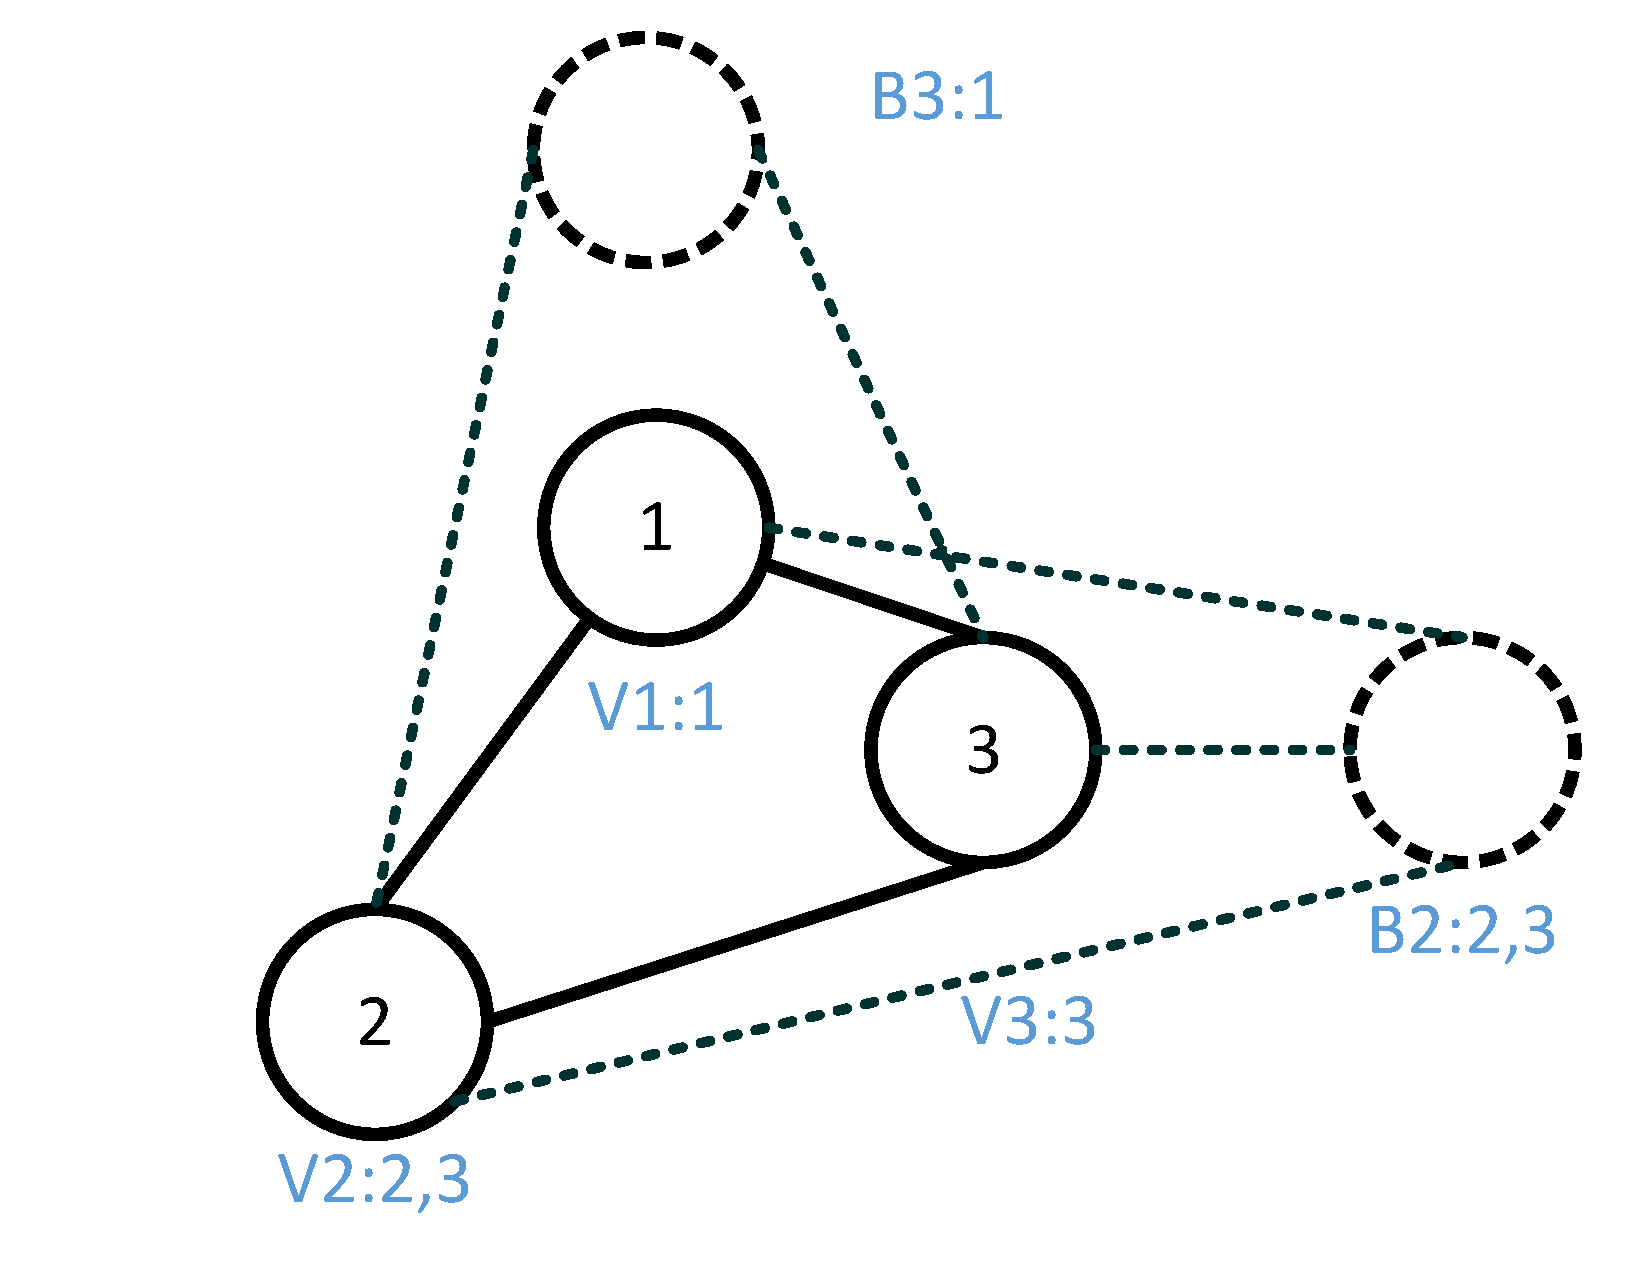
\includegraphics[width=1.5in]{Fig/nonoptgraph_SVNR}\\
\caption{non-optimal SVNR}\label{fig:nonoptgraphsvnr}
\end{figure}
\subsection{Survivable Virtual Network Request}
We would link some edges amongst nodes $V\cup B$ to construct 1-SNFT graph of arbitrary graph $G$ as show Fig.\ref{fig:optgraphsvnr},\ref{fig:nonoptgraphsvnr}, when only one node of VN failed, the former graph of VN is also subgraph isomorphism of graph of SVN. For example, when node v3 failed the node v2 run service 3 and backup node run service 2 so that the graph of VNR is subgraph isomorphism of SVN-v3 as shown in figure \ref{fig:optgraph_n1_fail},\ref{fig:optgraph_n2_fail},\ref{fig:optgraph_n3_fail},the red edge and red node is disable.

\begin{figure}
\centering
% Requires \usepackage{graphicx}
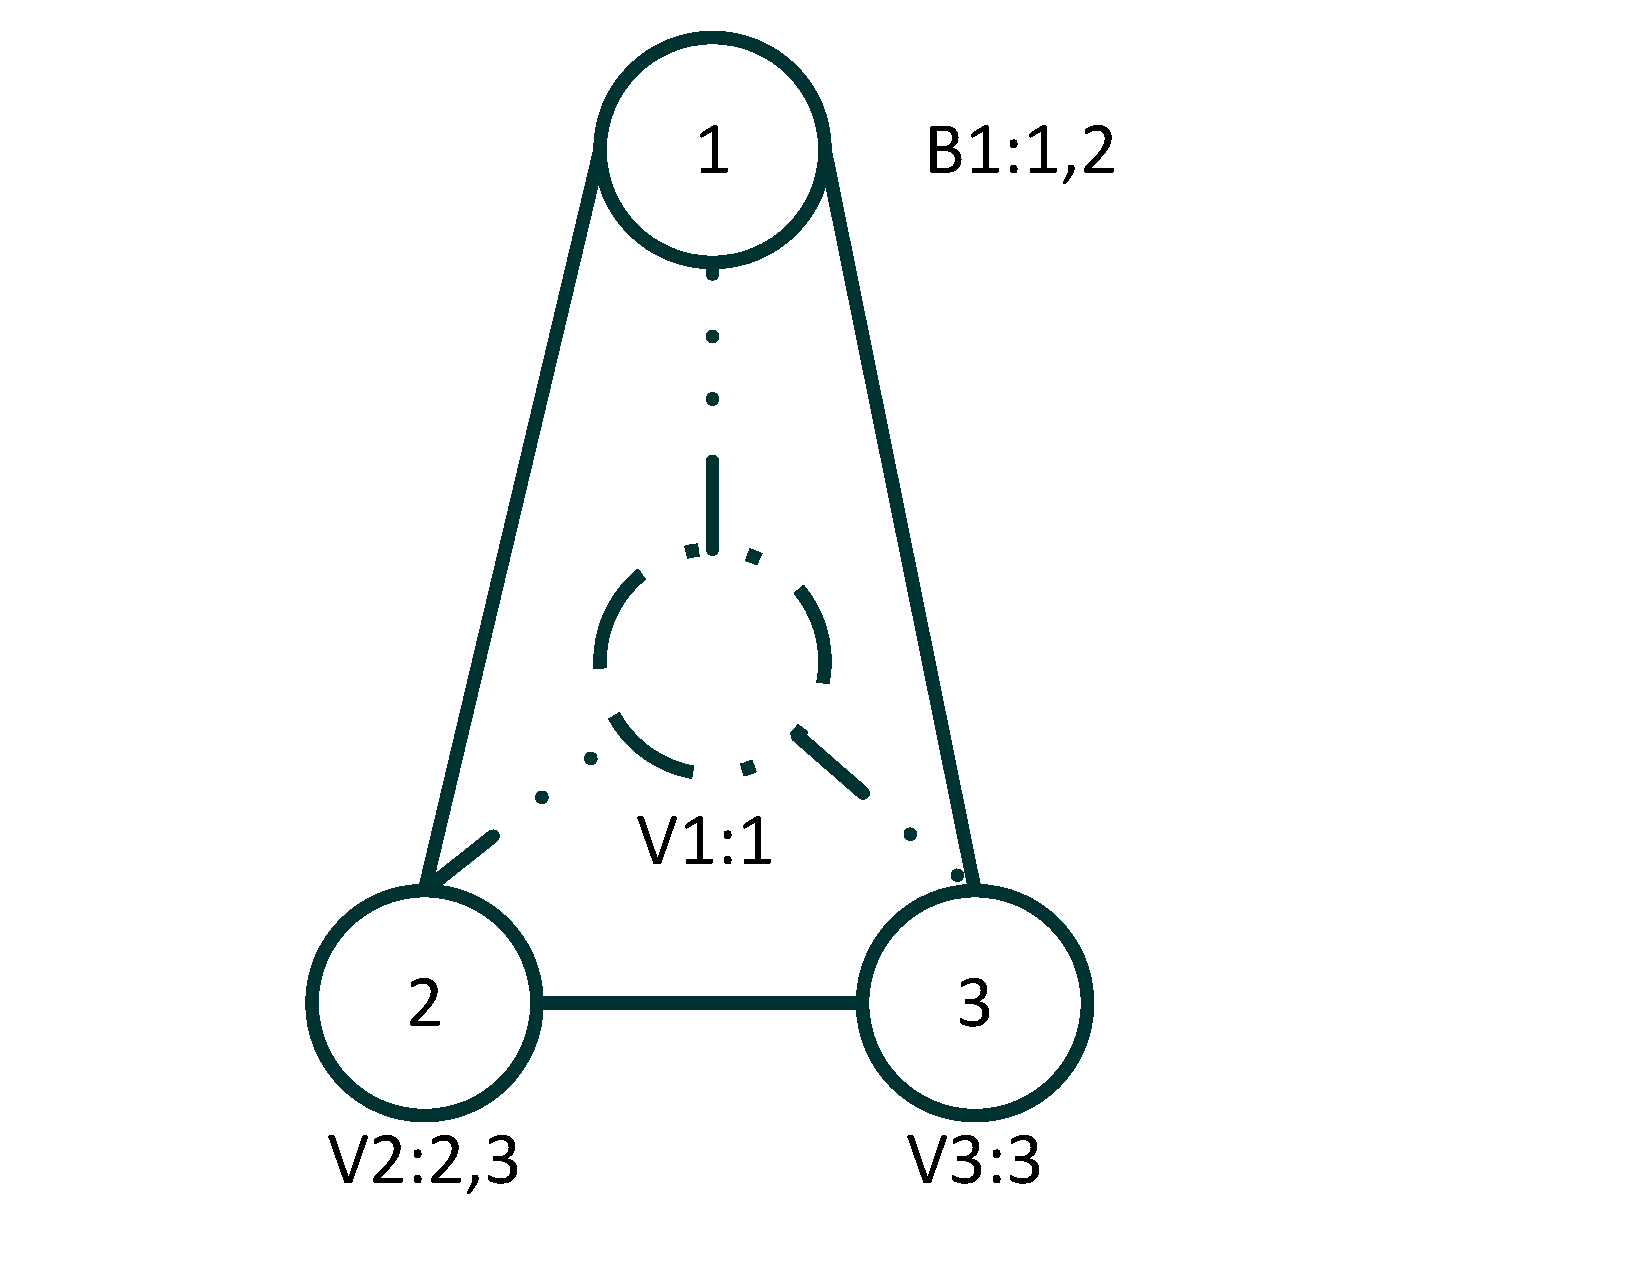
\includegraphics[width=1.5in]{Fig/SVNR_opt_n1}\\
\caption{node v3 failed in optimal SVNR}\label{fig:optgraph_n1_fail}
\end{figure}

\begin{figure}
\centering
% Requires \usepackage{graphicx}
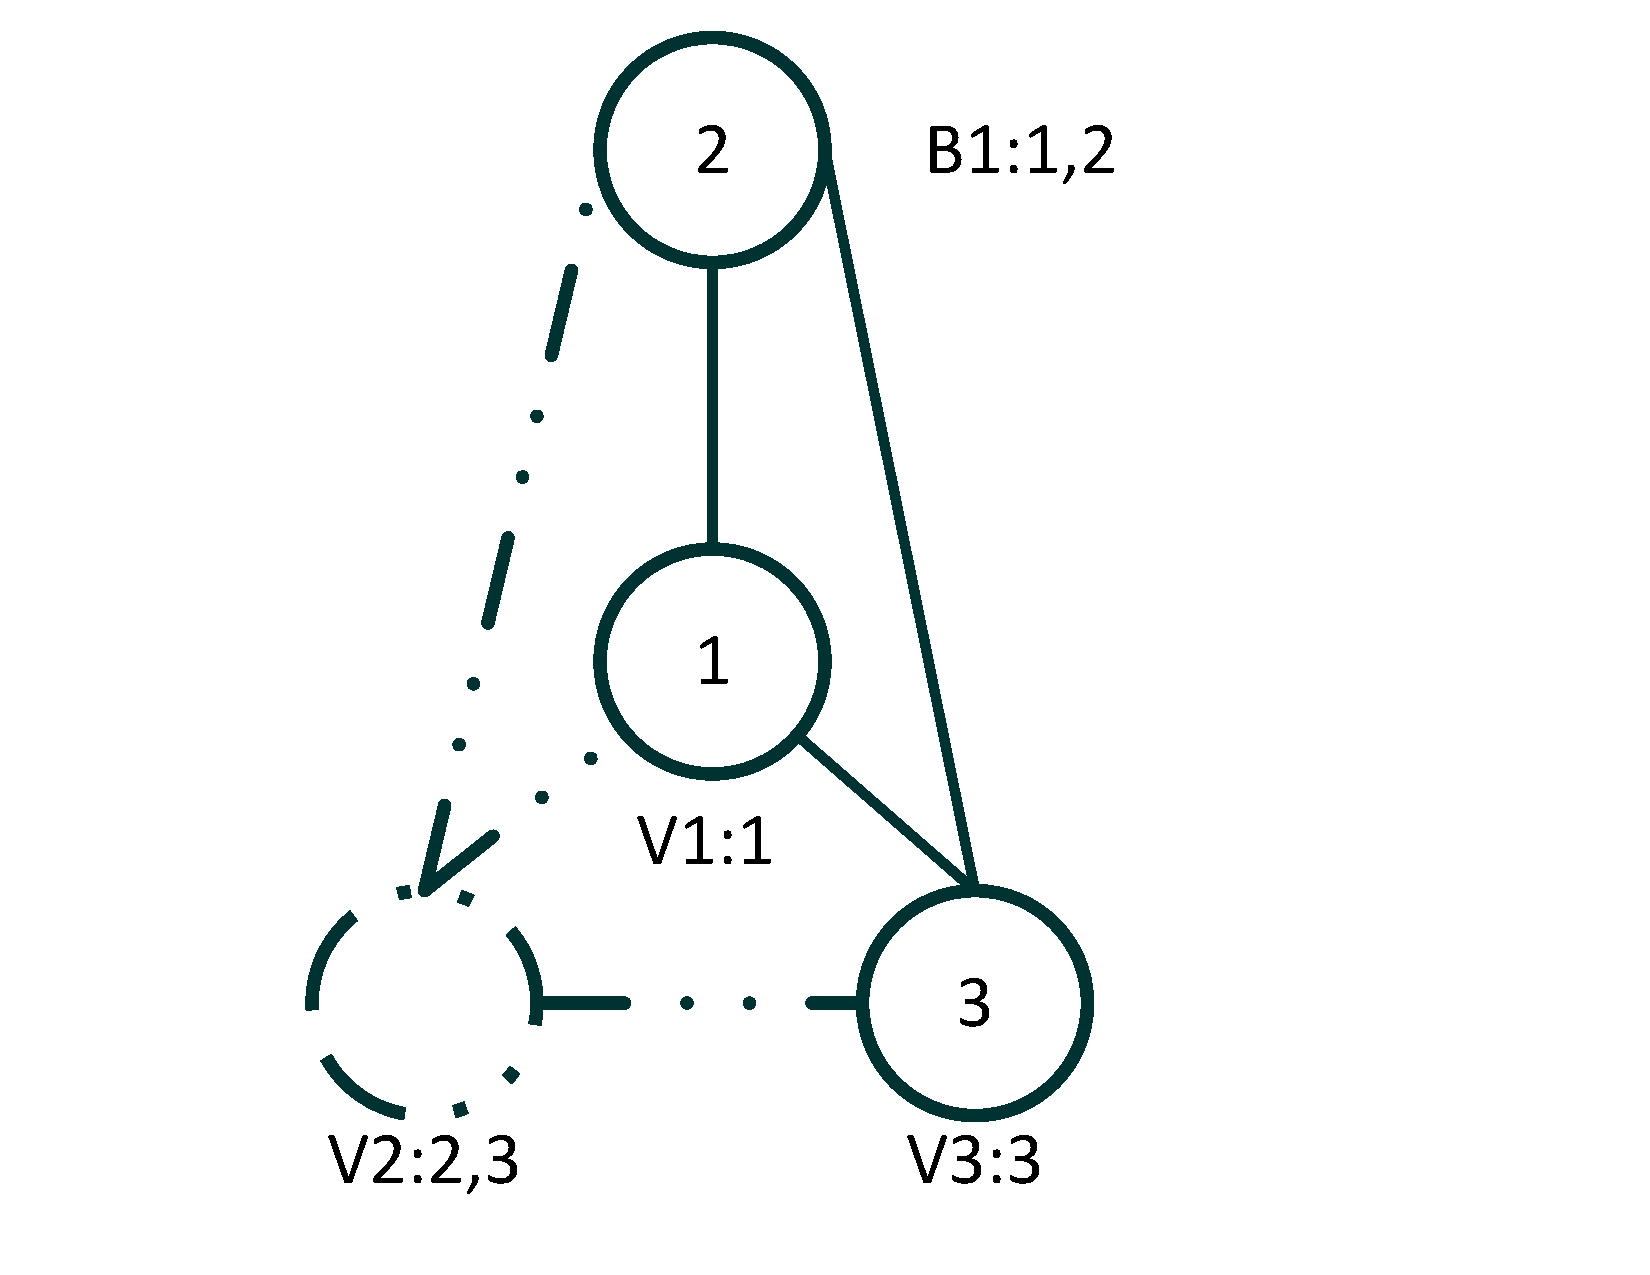
\includegraphics[width=1.5in]{Fig/SVNR_opt_n2}\\
\caption{node v3 failed in optimal SVNR}\label{fig:optgraph_n2_fail}
\end{figure}

\begin{figure}
\centering
% Requires \usepackage{graphicx}
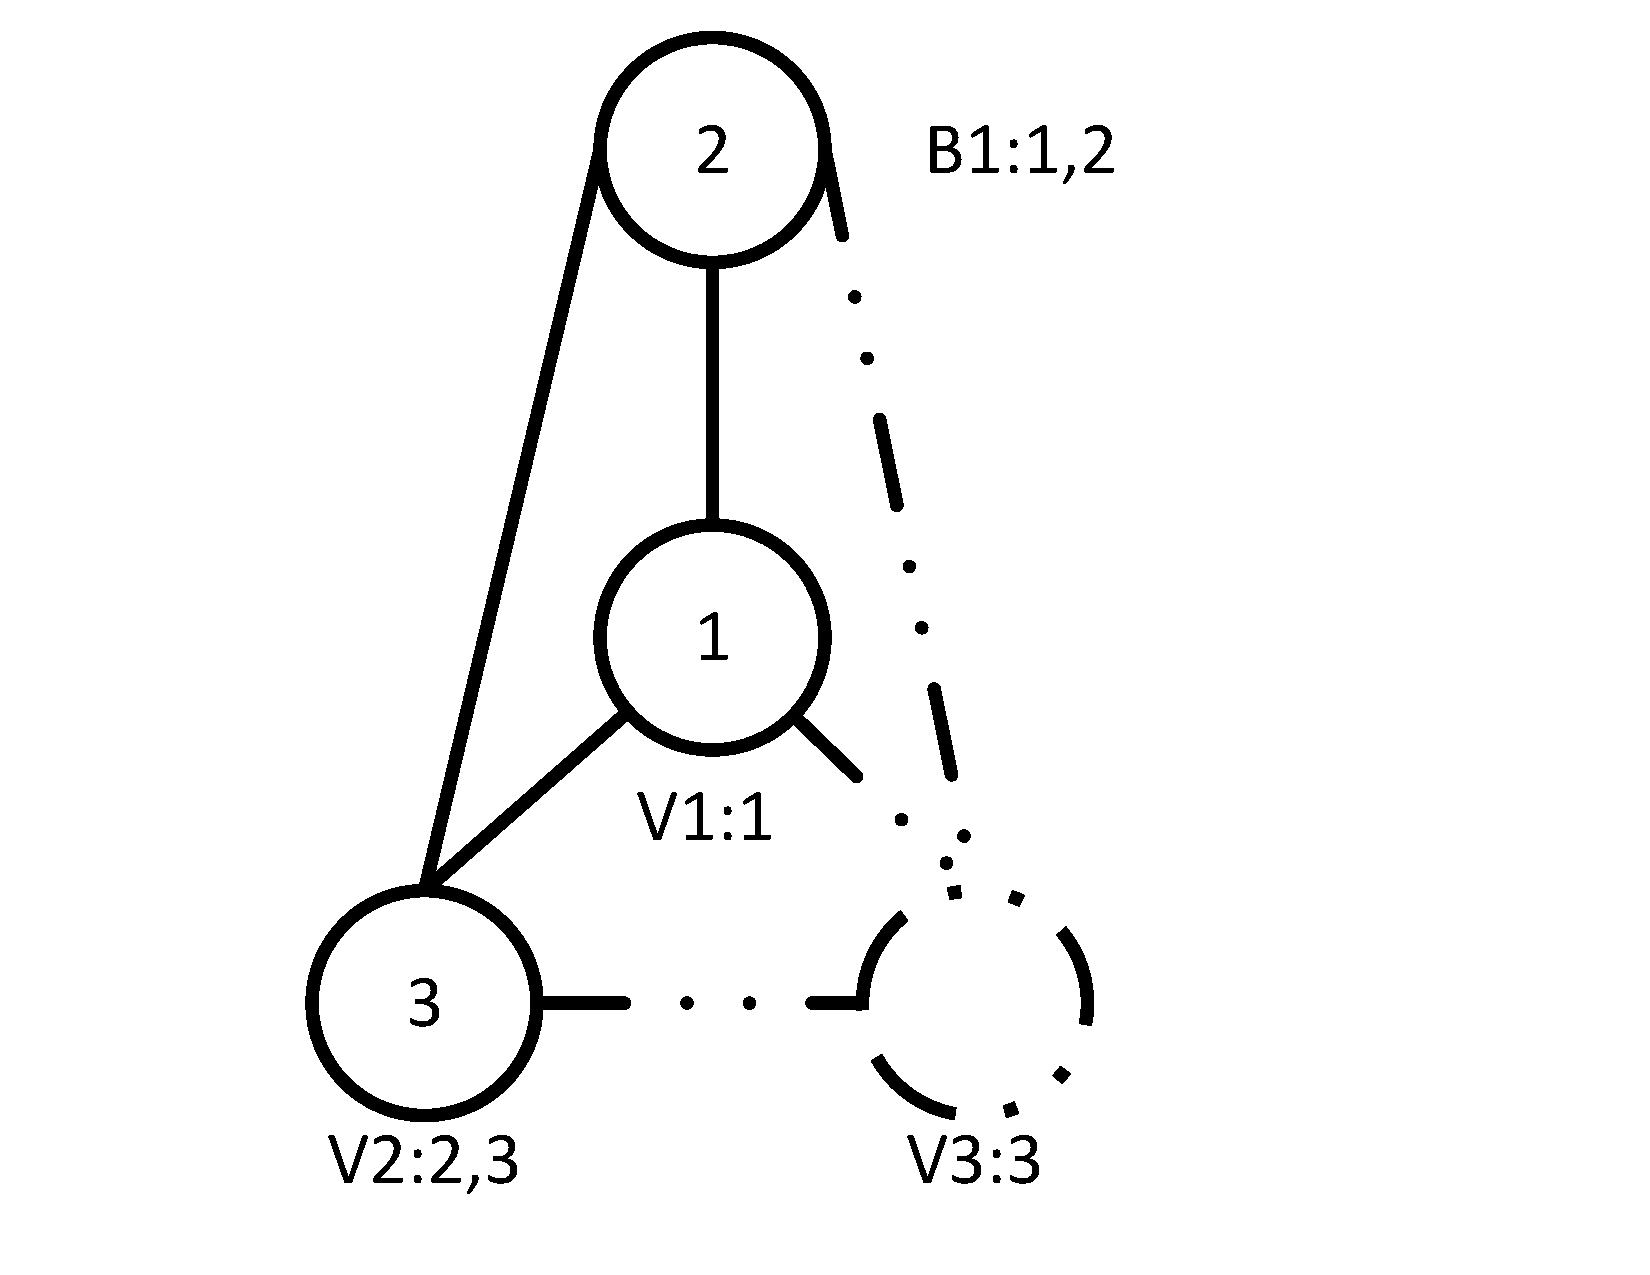
\includegraphics[width=1.5in]{Fig/SVNR_opt_n3}\\
\caption{node v3 failed in optimal SVNR}\label{fig:optgraph_n3_fail}
\end{figure}



It is our objection that firstly minimize number of added backup nodes, then minimize number of added edges to construct specific node fault tolerant graph. The graph of SVN, which is 1-NFT with node service function with respect to the graph of VN.



\subsection{Complexity of Problem}
\label{sec:Complexity}
this computation complexity of k-SNFT problem k-NFT($G(V,E,S)$) is NP, whose proof is below. when just exist one service function type in SVNR, the problem is degenerated into one-node fault-tolerant graph problem. when SVNR just have one type of service function, we must add only one backup node and add some edges into graph of VN to construct SVN, meantime the simplified problem is of equivalance to problem that one-node fault-tolerant graph problem which is NP.

when inserted node sets is previous given, the problem k-SNFT($G(V,E,S),B(V,S)$) is subproblem of k-SNFT($G(V,E,S)$).

Suppose topological structure of graph $G$ is path $P$, k-SNFT($P(V,E,S),B(V,S)$) is NP, the proof is below, exist one node n(n$\in V$) and we add backup nodes and edge to protect the node n, the former graph $P$ firstly is changed into $P+n$, nevertheless topological structure of $P+n$ may is not path, or be tree and non-tree graph. then protect other nodes of $V$.

the computation complexity of k-SNFT($T(V,E,S),B(V,S)$) is similarly available.

edge fault tolerant problem is subgraph of node fault tolerant problem
